\documentclass{article}
\usepackage{graphicx} % Required for inserting images
\usepackage{float} % Required for forcing figure placement
\usepackage{pgfplots}


\title{BigData Individual assignment 1}
\author{Ivan Anikin}
\date{October 2024}

\begin{document}

\maketitle



\section{Introduction}

\paragraph{Matrix multiplication is a fundamental operation in many fields of scientific computing, ML, and data analysis. Efficiency of matrix multiplication can vary significantly depending on the programming language, algorithm, and hardware environment used. In this assignment, I compare the performance of matrix multiplication across three programming languages—Python, C, and Java—using both intuitive approaches and optimized algorithms. }

\hfill 
\newline

\section{Performance comparison}

\begin{tabular}{| l | l | l | l |}
\hline
Metric & Python & C & Java \\ \hline
Execution time & 0.001007 s & 0.000000 s & 0.000000 s \\ \hline
Memory usage & 15.41 MB & 4.44 MB & 24 MB \\ \hline
CPU usage & 0.093750 s & 0.031250 s & 0.062000 s \\
\hline
\end{tabular}
\paragraph{Matrix size: 16x16}

\hfill 
\newline

\begin{tabular}{| l | l | l | l |}
\hline
Metric & Python & C & Java \\ \hline
Execution time & 0.481757 s & 0.015628 s & 0.032000 s \\ \hline
Memory usage & 17.48 MB & 4.964 MB & 25 MB \\ \hline
CPU usage & 0.578125 s & 0.046875 s & 0.062000 s \\
\hline
\end{tabular}
\paragraph{Matrix size: 128x128}

\hfill 
\newline

\begin{tabular}{| l | l | l | l |}
\hline
Metric & Python & C & Java \\ \hline
Execution time & 306.193860 s & 18.636116 s & 2.299000 s \\ \hline
Memory usage & 140.46 MB & 29.764 MB & 25 MB \\ \hline
CPU usage & 306.843750 s & 17.859375 s & 2.406000 s \\
\hline
\end{tabular}
\paragraph{Matrix size: 1024x1024}

\hfill 
\newline

\section{Performance analysis}

\paragraph{In terms of memory usage for 16*16 matrix, C is the most efficient, using only 4.44 MB compared to Python's 15.41 MB and Java's 24 MB. For CPU usage, Python exhibits the highest combined User + System CPU time (0.093750 seconds), followed by Java at 0.062000 seconds, while C remains the most efficient at 0.031250 seconds.}

\paragraph{As the matrix size increases to 128x128, the performance gap between the languages becomes more evident. C remains the fastest, with an execution time of only 0.015628 seconds, while Java takes 0.032 seconds, and Python lags behind at 0.481757 seconds.}

\paragraph{In terms of memory usage at 1024 matrix size, Python consumes the most (140.46 MB), while C uses 29.764 MB, and Java stays at 25 MB. Java also demonstrates superior CPU efficiency with 2.406000 seconds, compared to C’s 17.859375 seconds and Python’s 306.843750 seconds.}

\hfill 
\newline
\hfill 
\newline



\paragraph{Key Insights:}

\paragraph{
Execution Time: C performs exceptionally well on smaller matrices, but Java outperforms both Python and C significantly as matrix size increases, especially for larger matrices.
Memory Usage: C uses the least memory across all matrix sizes, followed by Python and then Java.
CPU Usage: Python consistently has the highest CPU usage, while C and Java are more efficient. Java particularly stands out in larger matrix sizes.
}

\paragraph{Based on these stats that I got by running the intuitive multiplication approach it seems, that the Python code is slowest while the C code is way faster. Both of them nevertheless seem to grow in cubic time regarding BigO. While Java seems closer to quadratic.}


\section{Multiplication time comparison charts}

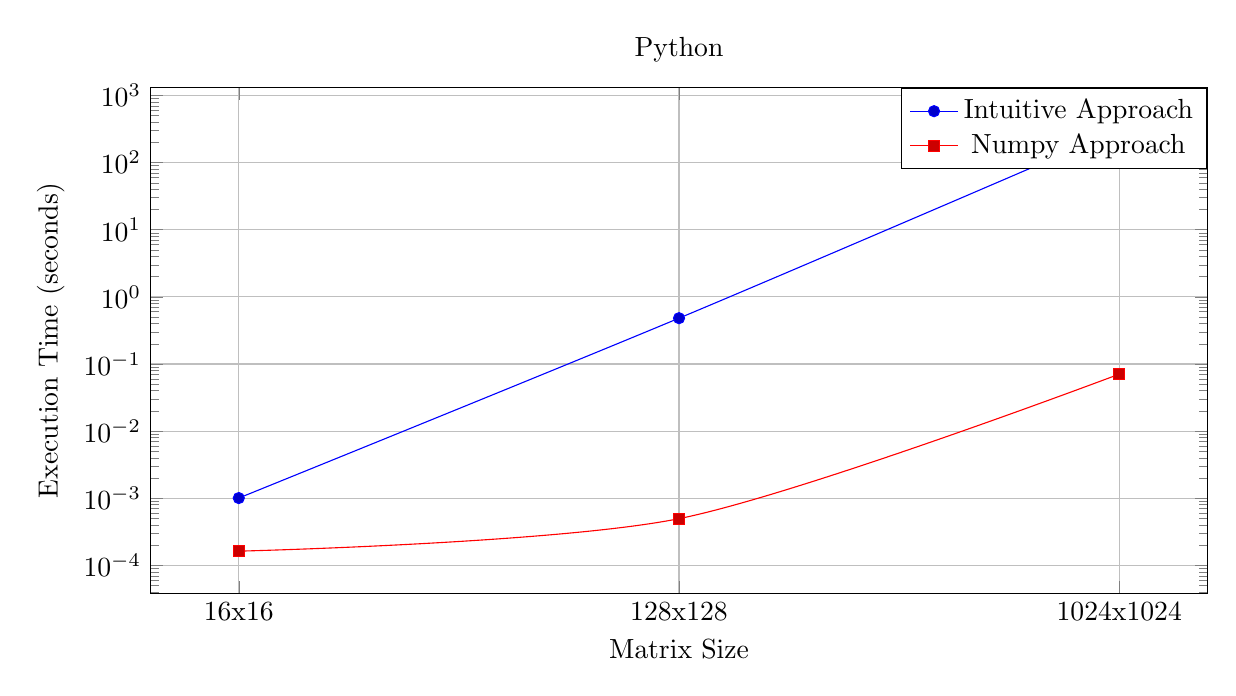
\begin{tikzpicture}
    \begin{axis}[
        width=15cm, height=8cm, % Increase the chart size
        title={Python},
        xlabel={Matrix Size},
        ylabel={Execution Time (seconds)},
        legend style={at={(1,1)}, anchor=north east},
        xtick={1, 2, 3},
        xticklabels={16x16, 128x128, 1024x1024},
        grid=major,
        ymode=log, % Use logarithmic scale for large differences in execution time
        smooth, % Make the lines smoother
        enlargelimits=true % Ensure that the plot is not cramped at the boundaries
    ]
    
    % Intuitive approach data
    \addplot coordinates {(1,0.001007) (2,0.481757) (3,306.193860)};
    \addlegendentry{Intuitive Approach}
    
    % Numpy approach data
    \addplot coordinates {(1,0.000163) (2,0.000497) (3,0.070671)};
    \addlegendentry{Numpy Approach}
    
    \end{axis}
\end{tikzpicture}


\paragraph{Python intuitive approach is slower than the Numpy implemented function taking using memory but at the same time moving the complexity from cubic to quadratic in BigO scale.}

\hfill 
\newline


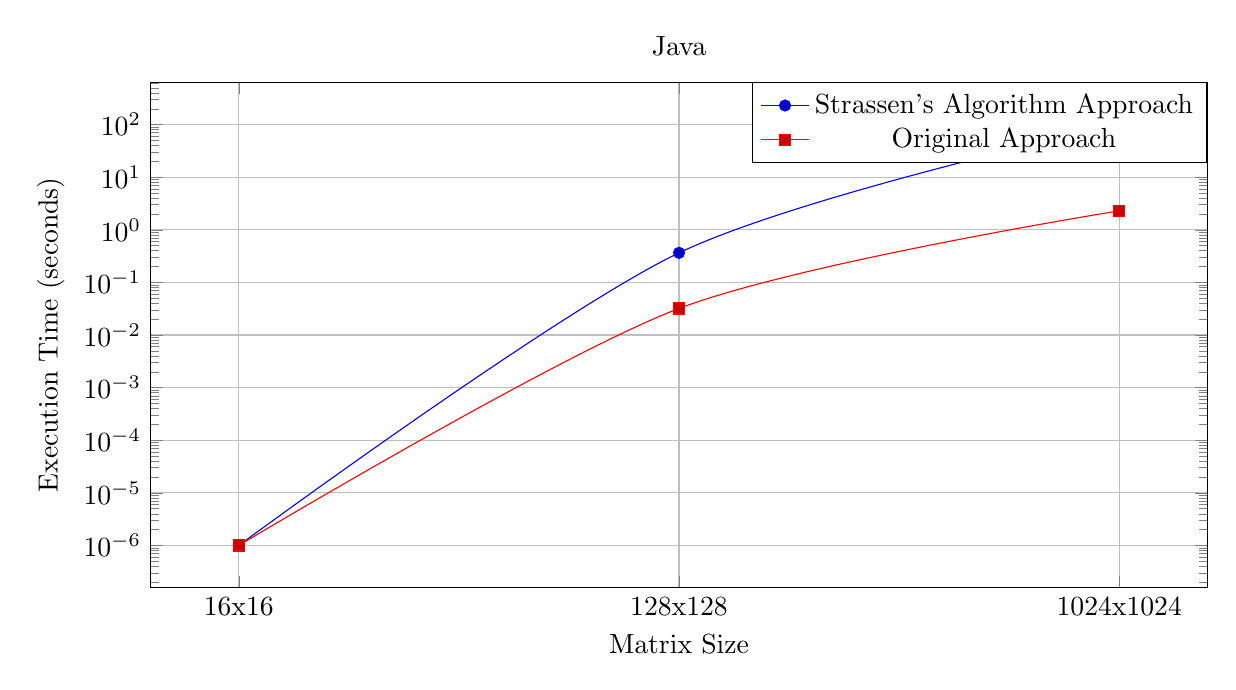
\begin{tikzpicture}
    \begin{axis}[
        width=15cm, height=8cm, % Larger size
        title={Java},
        xlabel={Matrix Size},
        ylabel={Execution Time (seconds)},
        legend style={at={(1,1)}, anchor=north east},
        xtick={1, 2, 3},
        xticklabels={16x16, 128x128, 1024x1024},
        grid=major,
        ymode=log, % Logarithmic scale for better comparison
        smooth,
        enlargelimits=true
    ]
    
    % New Java approach data
    \addplot coordinates {(1,0.000001) (2,0.365) (3,101.355)};
    \addlegendentry{Strassen's Algorithm Approach}
    
    % Original approach data
    \addplot coordinates {(1,0.000001) (2,0.032) (3,2.299)};
    \addlegendentry{Original Approach}
    
    \end{axis}
\end{tikzpicture}



\pagebreak

\section{Console log output stats}

\hfill 
\newline
\begin{figure}[H]
    \centering
    \includegraphics[width=1\linewidth]{image2.png}
\end{figure}
\paragraph{Multiplication using intuitive basic approach}

\hfill 
\newline
\begin{figure}[H]
    \centering
    \includegraphics[width=1\linewidth]{image.png}
\end{figure}
\paragraph{Multiplication using Numpy.matmul}



\hfill 
\newline
\begin{figure}[H]
    \centering
    \includegraphics[width=1\linewidth]{image3.png}
\end{figure}
\paragraph{Multiplication using intuitive basic approach}

\hfill 
\newline
\begin{figure}[H]
    \centering
    \includegraphics[width=1\linewidth]{image4.png}
\end{figure}
\paragraph{Multiplication using Strassen's Algorithm}


\end{document}


